\documentclass[xcolor=dvipsnames,t,aspectratio=169]{beamer} %t para ficar alinhado no topo do slide

\usecolortheme{rose}
\usecolortheme{dolphin}
\usetheme{Boadilla}

\usepackage[american]{babel}
\usepackage[utf8]{inputenc}
\usepackage{amsfonts}
\usepackage{amsmath}
\usepackage{amssymb}
\usepackage{latexsym}
\usepackage{graphicx}
\usepackage{listings} 
\usepackage{xcolor}
\usepackage{amsthm}
\usepackage{url}
\usepackage{textpos}
\usepackage{amssymb}
\usepackage{caption}
\usepackage{subcaption}
\usepackage{multicol}
\usepackage{mathrsfs}
\usepackage{float}
\setbeamersize{text margin left=1cm,text margin right=1cm,} 
\usepackage{pythonhighlight}
\usepackage{caption}
\usepackage{subcaption}
\usepackage{dsfont}
% \usepackage{natbib}

\setlength{\parindent}{0pt} % coloca identação no zero

\setbeamertemplate{itemize items}[circle]
\setbeamertemplate{itemize subitem}{$\blacktriangleright$}

\definecolor{fgv_dark_blue}{RGB}{1, 62, 125}
\definecolor{fgv_light_blue}{RGB}{6, 143, 203}
\setbeamercolor{normal text}{fg=fgv_dark_blue}\usebeamercolor*{normal text}


\setbeamercolor{title}{fg=fgv_dark_blue}
\setbeamercolor{frametitle}{fg=fgv_dark_blue}
\setbeamercolor{structure}{fg=fgv_dark_blue}
\setbeamercolor{author}{fg=fgv_light_blue}
\setbeamercolor{footline}{fg=fgv_dark_blue} 

\setbeamertemplate{footline}[frame number]
\setbeamertemplate{navigation symbols}{}

\definecolor{codegreen}{rgb}{0,0.6,0.2}
\definecolor{codegray}{rgb}{0.5,0.5,0.5}
\definecolor{codepurple}{rgb}{0.58,0,0.82}
\definecolor{backcolour}{rgb}{0.95,0.95,0.92}

\lstdefinestyle{mystyle}{
    backgroundcolor=\color{backcolour},   
    commentstyle=\color{codegreen},
    keywordstyle=\color{magenta},
    numberstyle=\tiny\color{codegray},
    stringstyle=\color{codepurple},
    basicstyle=\ttfamily\footnotesize,
    breakatwhitespace=false,  
    breaklines=true,                 
    captionpos=b,                    
    keepspaces=true,                 
    numbers=left,                    
    numbersep=5pt,                  
    showspaces=false,                
    showstringspaces=false,
    showtabs=false,                  
    tabsize=2
}

\lstset{style=mystyle}

\newcommand{\highlight}[1]{{\color{fgv_light_blue} #1}}

\newcommand{\ds}{\displaystyle}
\newcommand{\nl}{\newline}
\newcommand{\eps}{\varepsilon}
\newcommand{\ssty}{\scriptstyle}
\newcommand{\bE}{\mathds{E}}
\newcommand{\cB}{\mathcal{B}}
\newcommand{\cF}{\mathcal{F}}
\newcommand{\cA}{\mathcal{A}}
\newcommand{\cM}{\mathcal{M}}
\newcommand{\cD}{\mathcal{D}}
\newcommand{\cP}{\mathcal{P}}
\newcommand{\cN}{\mathcal{N}}
\newcommand{\cL}{\mathcal{L}}
\newcommand{\cLN}{\mathcal{LN}}
\newcommand{\bP}{{\rm I\!P}}
\newcommand{\bQ}{\mathbb{Q}}
\newcommand{\bN}{{\rm I\!N}}
\newcommand{\bR}{\mathds{R}}
\newcommand{\bZ}{\mathbb{Z}}
\newcommand{\bC}{\mathbb{C}}
\newcommand{\ind}{\mathds{1}}
\newcommand{\data}{\mathcal{D}}
\newcommand{\bV}{\mathds{V}}

% \renewcommand{\boldsymbol}{\symbf}

\newcommand{\bfP}{\boldsymbol{P}}
\newcommand{\bfQ}{\boldsymbol{Q}}
\newcommand{\bfX}{\boldsymbol{X}}
\newcommand{\bfY}{\boldsymbol{Y}}
\newcommand{\bfZ}{\boldsymbol{Z}}
\newcommand{\bfM}{\boldsymbol{M}}
\newcommand{\bfU}{\boldsymbol{U}}

\newcommand{\bfz}{\boldsymbol{z}}
\newcommand{\bfm}{\boldsymbol{m}}
\newcommand{\bfw}{\boldsymbol{w}}
\newcommand{\bfv}{\boldsymbol{v}}
\newcommand{\bfu}{\boldsymbol{u}}
\newcommand{\bfx}{\boldsymbol{x}}
\newcommand{\bfy}{\boldsymbol{y}}
\newcommand{\bfb}{\boldsymbol{b}}
\newcommand{\bfa}{\boldsymbol{a}}
\newcommand{\bfp}{\boldsymbol{p}}
\newcommand{\bff}{\boldsymbol{f}}
\newcommand{\tbx}{\tilde{\bfx}}
\newcommand{\tby}{\tilde{\bfy}}
\newcommand{\tbf}{\tilde{\bff}}
\newcommand{\yst}{\boldsymbol{y_\star}}
\newcommand{\fst}{\boldsymbol{f_\star}}
\newcommand{\xst}{\boldsymbol{x_\star}}
\newcommand{\bfth}{\boldsymbol{\theta}}
\newcommand{\bfmu}{\boldsymbol{\mu}}
\newcommand{\bfxi}{\boldsymbol{\xi}}
\newcommand{\bfsg}{\boldsymbol{\sigma}}


\newcommand{\htheta}{\hat{\theta}}
\newcommand{\poi}{\text{Poisson}}
% \newcommand{\var}{\text{Var}}
\newcommand{\cov}{\text{Cov}}
\newcommand{\gama}{\text{Gama}}
\newcommand{\normal}{\text{Normal}}
\newcommand{\ig}{\text{Inverse-Gamma}}
\newcommand{\ber}{\text{Bernoulli}}
\newcommand{\jg}{\text{Jg}}
\newcommand{\st}{\text{ s.t. }}
\newcommand{\otw}{\text{ otherwise }}
\newcommand{\sge}{\sigma_e^2}
\newcommand{\sgt}{\sigma_\theta^2}
\newcommand{\byi}{\bar{y}_i}
\newcommand{\gp}{\mathcal{GP}}

\newcommand{\dU}{\mathcal{U}}
% ---
% Baobá
\title{Gaussian Processes Visual Tool} %Published by {\color{fgv_light_blue} Stef van den Elzen} and {\color{fgv_light_blue}Jarke J. van Wijk} @ Eindhoven University of Technology}
\author{Eduardo Adame Salles\\
{\small\texttt{eduardo.salles@fgv.br}}\\
\vspace{0.4cm} \hspace{0.2cm} 
\includegraphics[scale = 0.25]{emap_logo}}

\date{{\color{fgv_dark_blue}  \textbf{Rio de Janeiro, Brazil}\\ \today}}

\begin{document}

\frame{\titlepage}

\addtobeamertemplate{frametitle}{}{%
\begin{textblock*}{200mm}(.88\textwidth,-.5cm)

\includegraphics[scale=0.15]{emap_logo}
\end{textblock*}}

\begin{frame}[c]{Introduction}

    \begin{block}{}
    GP Visual Tool is called to be a system for the interactive modeling, fitting and interpreting of \highlight{Gaussian processes}.
    \end{block}\vspace*{1cm}

    \begin{figure}[H]
        \centering
        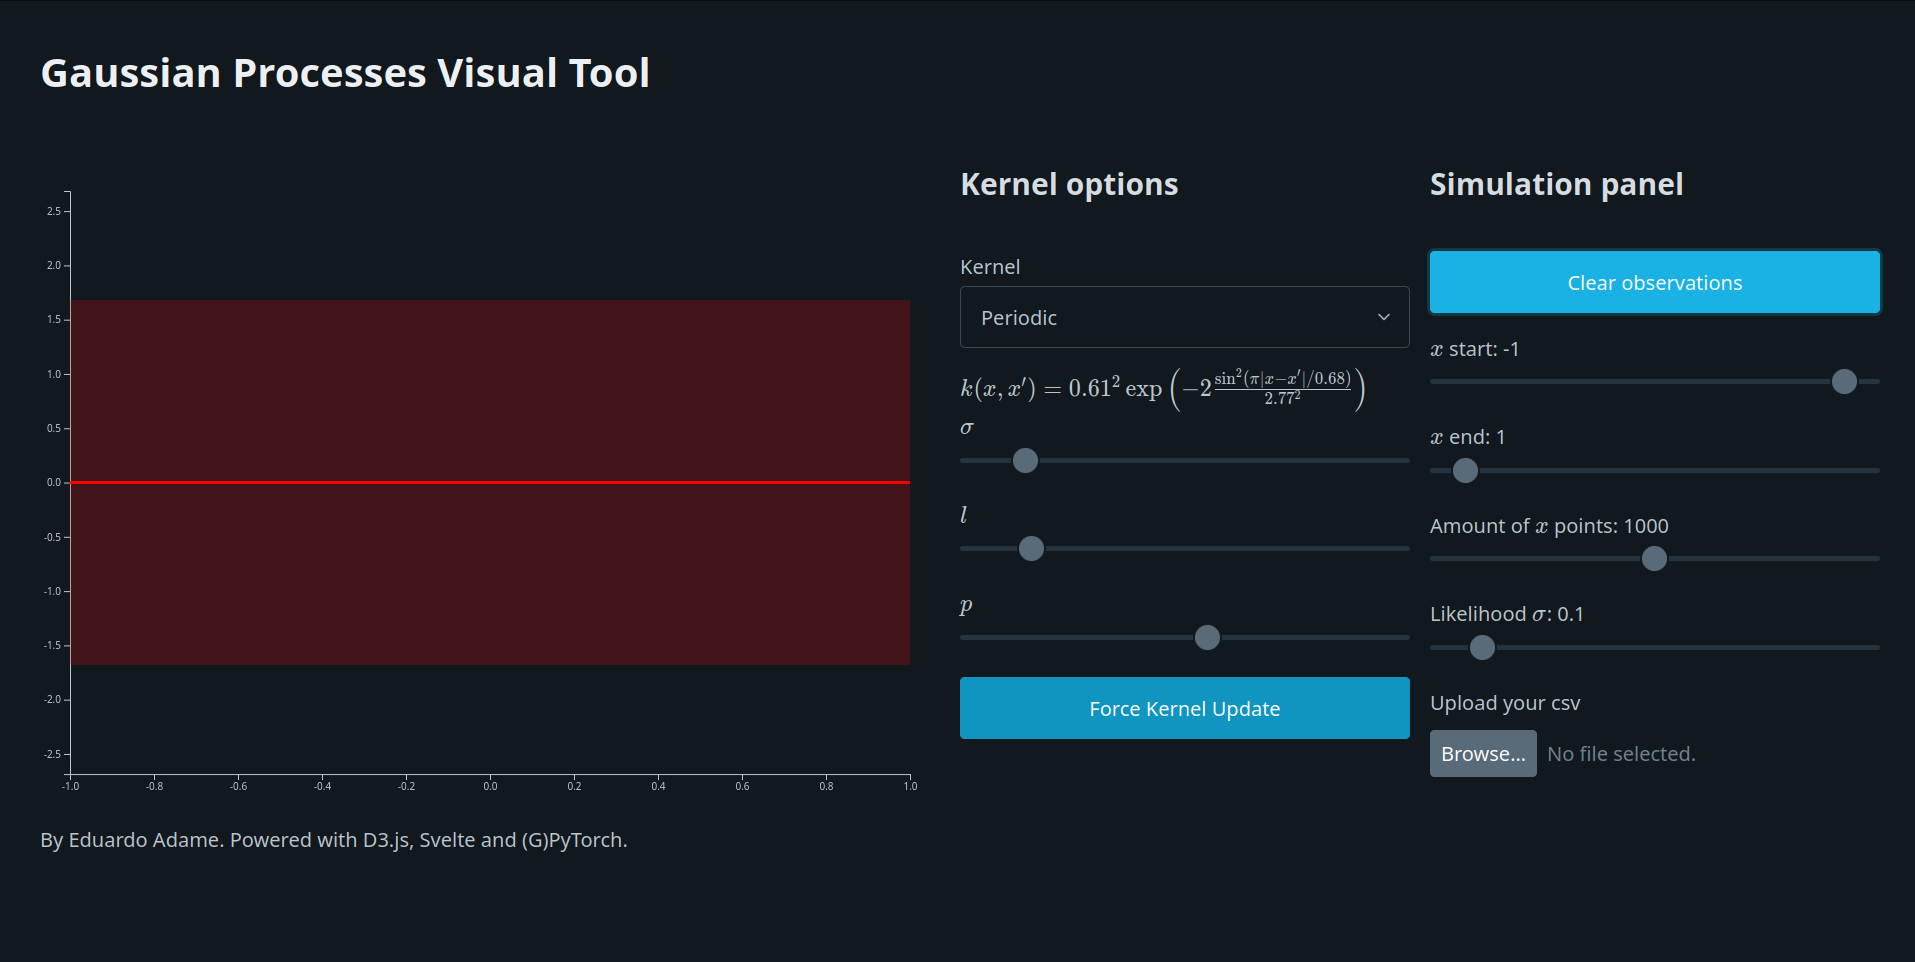
\includegraphics[height=.4\textheight]{../imgs/overall.png}
        \caption{Overall architecture of the system.}
    \end{figure}
    
    It allows the user to \highlight{rigorously} specify \highlight{a model} by choosing different sets of \highlight{hyperparameters}. 

\end{frame}

\begin{frame}[c]{What is a \highlight{Gaussian process}?}

Typically, \highlight{Gaussian processes} (GPs) can be seen as a generalization of the \highlight{Bayesian Regression}. Suppose we want to model a $f: \bR \to \bR$ as a GP. We would \highlight{define} it as following:

\begin{align*}
        \bfy \mid (\bff, \bfx) &\sim \cN(\bff, \sigma^2 I),\\
        \bff \mid \bfx &\sim \gp(m, k) \equiv \cN(m(\bfx), k(\bfx, \bfx)), 
    \end{align*}

    for $\bfx = x_1, \cdots, x_N$, $\bfy =  y_1, \cdots, y_N$ and $\bff =  f(x_1), \cdots, f(x_N)$. We often refer to $m$ as the \highlight{mean} function (usually $m(x_i) = 0$) and $k$ as the \highlight{kernel} function. Our goal is to find the \highlight{\textit{posterior} distribution} of $f$.

\end{frame}

\begin{frame}[c]{\highlight{Means} and \highlight{Kernels}}
    In order to define our \textit{priors} distributions, we need to specify the \highlight{mean} and \highlight{kernel} functions. The \highlight{mean} function is usually set to zero, but the \highlight{kernel} function is a bit more complicated.

    There are some properties of kernels:
    \begin{itemize}
        \item \highlight{Symmetry}: $k(x, x') = k(x', x)$;
        \item \highlight{Positive definiteness}: $\sum_{i=1}^n \sum_{j=1}^n c_i c_j k(x_i, x_j) \geq 0$ for any $n \in \bN$, $c_1, \cdots, c_n \in \bR$ and $x_1, \cdots, x_n \in \bR$;
        \item \highlight{Stationarity}: $k(x, x') = k(x - x')$;
        \item \highlight{Isotropy}: $k(x, x') = k(\|x - x'\|)$.
    \end{itemize}
\end{frame}

\begin{frame}[c]{Finding the \highlight{\textit{posterior} distribution}}
    Fitting a GP to a dataset is equivalent to finding the \highlight{\textit{posterior} distribution} of $f$ given $\bfy$ and $\bfx$. This is done by using \highlight{Bayes' theorem}:

    \begin{align*}
        p(\bff \mid \bfy, \bfx) &= \frac{p(\bfy \mid \bff, \bfx) p(\bff \mid \bfx)}{p(\bfy \mid \bfx)}\\
        &= \frac{p(\bfy \mid \bff, \bfx) p(\bff \mid \bfx)}{\int p(\bfy \mid \bff, \bfx) p(\bff \mid \bfx) d\bff}\\
        &= \frac{p(\bfy \mid \bff, \bfx) p(\bff \mid \bfx)}{\int p(\bfy \mid \bff, \bfx) p(\bff \mid \bfx) d\bff}\\
        &\propto p(\bfy \mid \bff, \bfx) p(\bff \mid \bfx)\\
        &\propto \cN(\bfy \mid \bff, \sigma^2 I) \cN(\bff \mid \bfx, k(\bfx, \bfx)).
    \end{align*}
\end{frame}

\begin{frame}[c]{Some \highlight{approaches} to get \highlight{optimal} hyperparams}

    As much of the work in the field of Bayesian statistics, we need to specify \highlight{priors} for our hyperparameters. This is usually done by using \highlight{Gamma} and \highlight{Inverse Gamma} distributions. But somewhere we have to choose the \highlight{hyperparameters}.

    Maximizing the evidence is a common approach to get the \highlight{optimal} hyperparameters. This is done by maximizing the \highlight{log-marginal likelihood}:

    \begin{align*}
        \log p(\bfy \mid \bfx) &= \log \int p(\bfy \mid \bff, \bfx) p(\bff \mid \bfx) d\bff\\
        &= \log \cN(\bfy \mid \bfx, k(\bfx, \bfx) + \sigma^2 I).
    \end{align*}

    
\end{frame}

\begin{frame}[c]{Applications of \highlight{GPs}}
    As any Machine Learning model, GPs can be used in a wide range of applications. Some of them are:

    \begin{itemize}
        \item Emulating \highlight{expensive} functions;
        \item \highlight{Regression} problems;
        \item \highlight{Classification} problems;
        \item \highlight{Time series} prediction;
        \item Anomaly \highlight{detection};
    \end{itemize}

    And some of its \highlight{advantages} are:
    \begin{itemize}
        \item \highlight{Uncertainty} estimation;
        \item \highlight{Interpretability};***
        \item \highlight{Flexibility}.
    \end{itemize}
\end{frame}

\begin{frame}[c]{Life \highlight{could} be a dream.}
    %Limitations

    As one would say, \highlight{there is no free lunch}. GPs are not an exception. Some of its \highlight{limitations} are:

    \begin{itemize}
        \item \highlight{Computational} complexity;
        \item \highlight{Memory} requirements;
        \item \highlight{Non-convex} optimization;
    \end{itemize}
\end{frame}

\begin{frame}[c]{Developing a \highlight{visual} tool}
    In order to understand the behavior of GPs, and each decision we make, a \highlight{visual} tool could be very useful. That's when Gaussian Processes Visual Tool comes in.

    We want to, but not limited to:

    \begin{itemize}
        \item \highlight{Visualize} the behavior of GPs;
        \item Add new observations \highlight{interactively};
        \item Change the \highlight{kernel} function;
        \item \highlight{Choose} hyperparameters in real-time;
        \item Use our own custom \highlight{datasets};
    \end{itemize}
\end{frame}

\begin{frame}[c]{Technologies}
    In order to develop this tool, we will use:

    \begin{itemize}
        \item \highlight{Python} and \highlight{Javascript} as programming languages;
        \item \highlight{PyTorch} and \highlight{GPyTorch} to handle the GPs;
        \item \highlight{Flask} to \highlight{serve} our application;
        \item \highlight{D3.js} to deal with the \highlight{visualizations};
        \item \highlight{Svelte} to give us a \highlight{reactive} frontend;
    \end{itemize} 
    
\end{frame}

\begin{frame}[c]{Let's start \highlight{sampling}}
    Our main interactive visualization is a \highlight{line plot} of the current GP. We can \highlight{sample} from it by clicking on any point of the plot. This will add a new point to the plot, and a new sample to the \highlight{posterior} distribution. Clicking in an existing point will remove it from the plot, and the sample from the posterior.

    \begin{figure}[H]
        \centering
        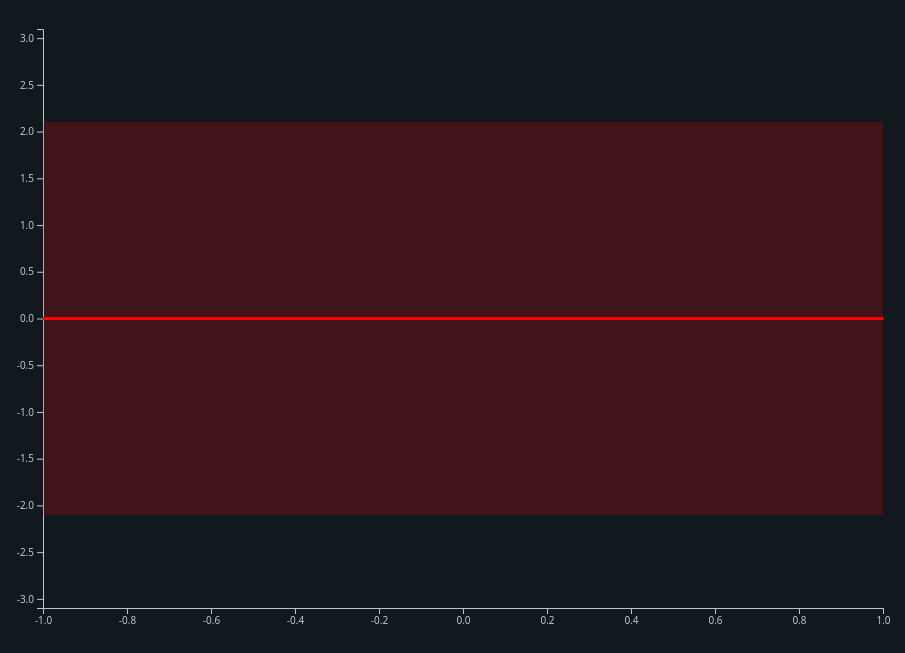
\includegraphics[width=0.4\textwidth]{../imgs/observing.png}
        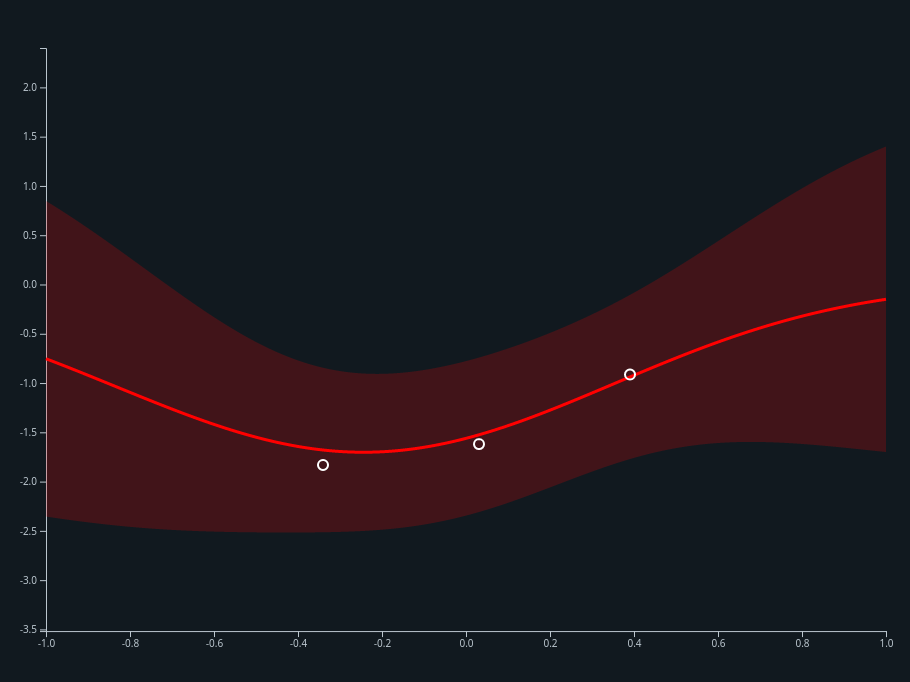
\includegraphics[width=0.39\textwidth]{../imgs/observed.png}
        \caption{Sampling from the GP.}
    \end{figure}

    Hovering, you can see the \highlight{marginal} distribution of the point.
\end{frame}

% \begin{frame}[c]{Some \highlight{marginals} are not that bad\footnote{Marginal distributions :D}}
    
% \end{frame}

\begin{frame}[c]{Beyond \highlight{choosing} a kernel}
    As we said before, we can change the kernel function. We can also change the \highlight{hyperparameters} of the kernel. This will change the \highlight{behavior} of the GP.

    \begin{figure}[H]
        \centering
        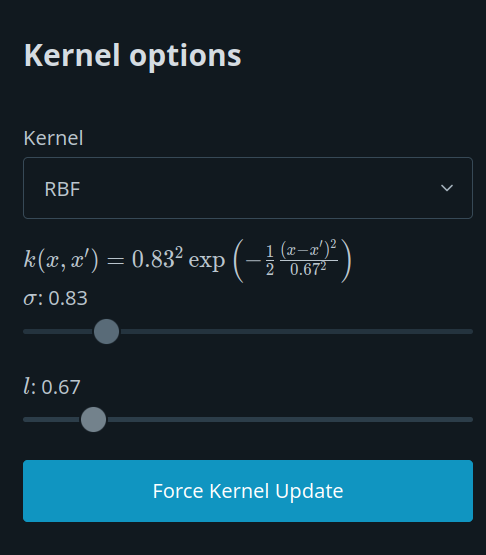
\includegraphics[width=0.30\textwidth]{../imgs/kernel-1.png}
        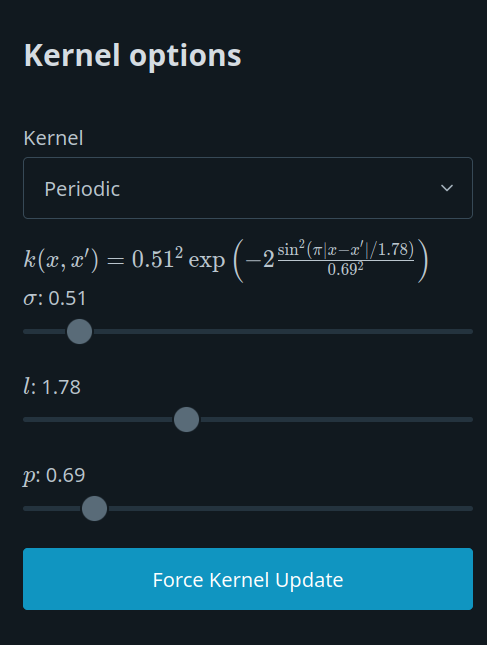
\includegraphics[width=0.26\textwidth]{../imgs/kernel-2.png}
        \caption{Changing kernels.}
    \end{figure}

\end{frame}

% \begin{frame}[c]{Math is actually \highlight{important}}
    
% \end{frame}

\begin{frame}[c]{Customization \highlight{is} allowed}
    \begin{multicols}{2}
    You can also \highlight{upload} your own dataset. This will allow you to \highlight{play} with the tool, and see how the GP behaves with your own data. You can set the \highlight{noise} level, and axis \highlight{limits}.

    \begin{figure}[H]
        \centering
        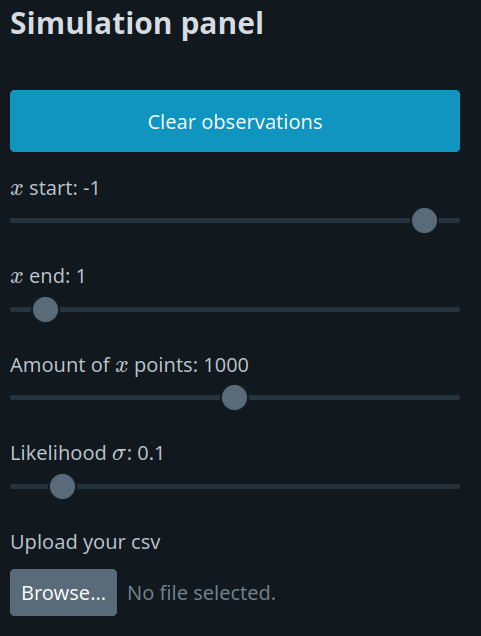
\includegraphics[width=0.30\textwidth]{../imgs/simulation.png}
        \caption{Simulation options}
    \end{figure}
    \end{multicols}
\end{frame}

\begin{frame}[c]{Future \highlight{work}}
    There are some things we would like to add to the tool:

    \begin{itemize}
        \item Add \highlight{more} visualizations, like a heatmap of the covariance matrix;
        \item Add more \highlight{kernels};
        \item Include \highlight{export} options;
        \item Make it run on \highlight{GPU} by default;
        \item Deploy it to a \highlight{server};
        \item Add math \highlight{explanations} to the tool;
        \item Operations between \highlight{kernels};
    \end{itemize}
    
\end{frame}

\begin{frame}[c]
\frametitle{~}
    
    \begin{center}
        {\Huge Thanks!}
    \end{center}
    
\end{frame}





\end{document} 